\section{(Distributed) Denial of Service Attacks}

\paragraph{Denial of Service Attack}
Making a service or network resource unavailable to its intended / legitimate users. Typically achieved by exhausting available resources by sending an excessive amount of traffic.

To mitigate such attacks, it is common to use a combination of various mitigation techniques at different points in the network hierarchy.

First, an attack has to be detected (by comparing it to normal / human traffic patterns) and then it has to be filtered.

\paragraph{Distributed DoS Attack}
Many different sources simultaneously (often with botnets). Often used to extort companies. Harder to track and take down than a regular DoS attack and also easier to hide identity. Allows for a virtually unlimited bandwidth for flood attacks.

\paragraph{Attack Targets}
See Figure \ref{fig:ddos_target} for an overview.

\begin{figure}[h]
	\centering
	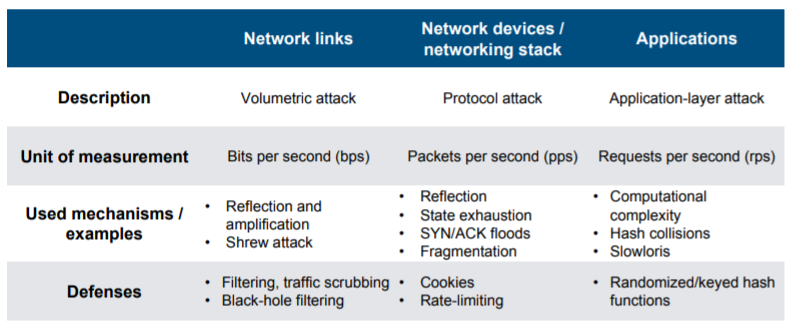
\includegraphics[scale=0.7]{images/910-targets.PNG}
	\caption{Targets of a (D)DoS attack.}
	\label{fig:ddos_target}
\end{figure}

\subsection{General DoS Attack Techniques}

\paragraph{Features Facilitating DoS Attack}
\begin{itemize}
    \item Attacker controls significantly more resources than victim.
    \item Attacker needs to expend significantly less resources than victim.
    \item Attacker can hide his identity / continually change it.
    \item Victim needs to expend a significant amount of resources before being able to assess the legitimacy of requests.
    \item Attacker can instruct / trick other entities to send traffic on their behalf.
\end{itemize}

\begin{figure}[h]
	\centering
	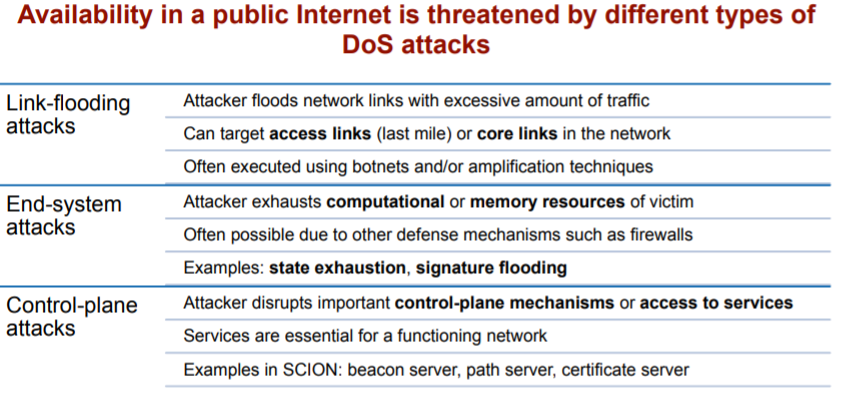
\includegraphics[scale=0.6]{images/910-attacks.PNG}
	\caption{Different kinds of DoS attacks.}
	\label{fig:attacks}
\end{figure}

\paragraph{(IoT) Botnets}
A (large) set of compromised machines (often IoT devices) connected to the Internet. They execute malicious code and can be controlled via command and control (C\&C) systems. They are often geographically distributed.

Components: command and control infrastructure to push commands to bots (often owned by attackers), zombies = devices under control of the attackers (often vulnerable hosts infected by malware) and bots - software that contains the malicious business logic.

To spread, an infected device will scan and look for open ports (e.g. sending TCP-SYN packets to randomly generated IP addresses), brute force a login, report target to controller and infect by connecting to found device and uploading malware.

IoT devices since you can have many with uniform configuration (configure-and-forget), are poorly secured (e.g. default credentials), not regularly updated (in regards to security) and often connected to the Internet without bandwidth limitations.

E.g.: Mirai botnet (mostly vulnerable webcams).

\textbf{Mitigations:} patching (automatic security updates for the device's full lifetime), credentials (not hardcoded and forced to change default passwords), monitoring (ISPs should actively monitor network for suspicious traffic).

\paragraph{Reflection and Amplification}
Need publicly accessible servers and the ability to spoof source address. Ideally, the responses caused should be (much) larger than the requests (amplification). Can be combined with a botnet consisting of master and agent nodes to exponentially grow volume.

Typical reflectors are: DNS (max. amplification 180), NTP (max. amplification 500) and Memcached (max. amplification 50'000) \footnote{Currently, NTP vulnerability is closed along with Memcached having UDP disabled.}.

An example DNS query that triggers a big response is the ANY query - it returns all DNS records of a domain (including the lengths SOA records). Nowadays, most DNS resolvers / authoritative servers refuse to respond to ANY queries or limit the response size.

\textbf{Amplification factor:} response bytes / request bytes. 

\textbf{How to:}
\begin{itemize}
    \item Choose open service as reflector (e.g. open DNS resolver).
    \item Craft a request that triggers (much) larger response.
    \item Send packet where source address is set to victim's address.
    \item Reflector sends reply to victim.
\end{itemize}

\textbf{Mitigations:} perform access control, implement response rate limiting (RRL) and ensure small amplification factors (ideally $< 1$)\footnote{WireGuard ensures that the responder's first message is smaller than the initiator's.}.

\paragraph{Address Spoofing}
Source address in an IP header can be set by the sender and in a connectionless protocol, such as UDP, a server cannot confirm the actual sender.

\textbf{Defenses:} Address filtering by ISPs (hosts should use their own addresses - would need to be globally deployed and the incentives are poor since only other ISPs profit), using connection-based protocols (such as TCP - comes with additional latency and other ways to DoS (state exhaustion)) and cryptographic source authentication (again, other attack possibilities if asymmetric crypto and requires symmetric key distribution / PKIs).

\begin{figure}[h]
	\centering
	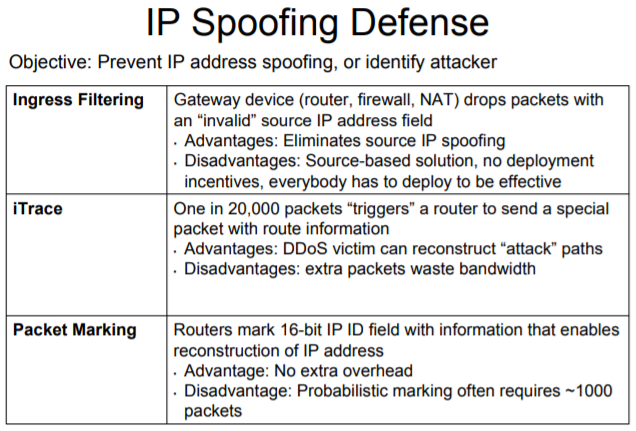
\includegraphics[scale=0.7]{images/910-ipspoof.PNG}
	\caption{IP spoofing defenses.}
	\label{fig:ipspoof}
\end{figure}

\subsection{Specific Attack Examples}

\paragraph{Volumetric: Shrew Attack}
Achieving the same effect of bandwidth-based DoS (high-rate attack traffic) with low-rate attack traffic by exploiting the TCP congestion control feature (exponential backoff if packet loss is detected).

Periodically sending short bursts to the target link / router denies the bandwidth of legitimate TCP flows at it makes TCP believe there is a long-term congestion. The bursts are most commonly send exactly when client is trying to send legitimate traffic (MITM attack in this case since the attack needs to be coordinated).

\textbf{Temporal lensing:} concentrating a low-bandwidth flood into a short, high-bandwidth pulse s.t. even a low-bandwidth attacker can perform a shrew attack. By knowing the attack path latencies, e.g. from reflector to victim, the attacker can send packets at different times to reflectors with varying path latencies s.t. overall traffic arrives at victim at the same time. With lensing, attackers can achieve peak bandwidths larger than their actual upload bandwidth. Lensing can be combined with amplification to create even larger pulses.

\paragraph{Volumetric: Coremelt}
Adversary controls botnet distributed across Internet. Bots send traffic between each other (not to victim, desired traffic). Adversary exhausts bandwidth on victim link in a per-flow fair sharing system.

\paragraph{Volumetric: Crossfire}
Adversary controls botnet distributed across Internet. Since route optimization leads to few links actually being used to target a region to rest of the Internet, adversary can contact selected servers to overload these links. Can disconnect target region from remainder of Internet.

\paragraph{Protocol: DNS Flooding / NXDOMAIN Attack}
Overwhelm the victim's authoritative name servers by querying many non-existent subdomains of victim domain. The DNS resolvers query all authoritative name servers in turn and thus a name server will not reply to legitimate requests. The more attackers and resolvers the better.

\paragraph{Protocol: Session State Exhaustion}
Two-way communication channels are identified with unique session numbers (= session state). Numbers are known at a server to match subsequent requests to right session. By exhausting the session state table of the server, it can no longer accept new connections, existing connections are dropped and maybe the server / service even crashes.

\textbf{Generic mitigations:} Encode state in a unique but determined way that allows server to validate state in client reply. No state at server is needed (other than salt). Ensure the encoding cannot be tampered (use crypto-hashes, unique data known to server only and changes over time, etc.), e.g. $B =$ Hash(salt, $A$).

\textbf{SYN flood attack:} TCP three-way handshake first message is client sending a SYN packet with a random sequence number $A$ and server keeps $A+1$ and $B$ (random seq. number of server SYN+ACK). With spoofed source addresses, a server can be flooded with SYN messages and the state table will eventually overflow.

\textbf{SYN flood attack mitigation:} SYN cookies - no state tables needed if initial TCP sequence number is particularly chosen (e.g. $B = F(\text{time, IP address, port, ...})$. Apply $F$ after ACK of client to validate and establish connection.

\paragraph{Application-Layer: Algorithmic Complexity}
Induce the worst-case behavior in a vulnerable algorithm. The larger the difference between worst and average case, the more vulnerable it is. See Figure \ref{fig:complex} for a comparison.

\begin{figure}[h]
	\centering
	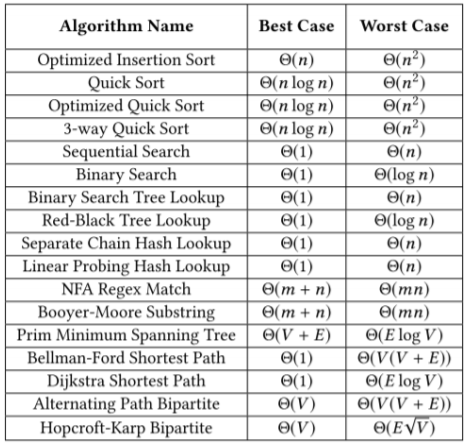
\includegraphics[scale=0.7]{images/910-complex.PNG}
	\caption{Comparison of best and worst case complexities.}
	\label{fig:complex}
\end{figure}

\textbf{Hash table lookup collisions:} collisions are common due to small size. Resolutions include chaining, open addressing, etc. An attacker can intentionally pick a bad input sequence that causes worst-case hash table collisions. Countermeasures include universal hashing (guaranteed zero to little collisions for any input), hash randomization (hard to find bad input), etc. %TODO: more?

\textbf{Regular Expression DoS (ReDoS):} provide a regular expression that takes a very long time to evaluate (matching). Most regex implementations have exponential time worst case complexity - meaning that the time taken can grow exponentially in relation to input size.

\paragraph{Application-Layer: Slowloris}
A single machine can take down another machine's web server with minimal bandwidth by:
\begin{itemize}
    \item Keeping many connections to target web server open and holding them open as long as possible.
    \item Opening connections and sending partial requests.
    \item Periodically sending subsequent HTTP headers adding to the request but never completing it.
\end{itemize}
Affected servers will keep these connections open, filling their maximum concurrent connection pool and eventually denying additional ones. 

\textbf{Mitigations:} increase max. possible connections to server, limiting connections from single IP address source, require minimum transfer speed per connection, restrict length of time client is allowed to stay connected. Or: set up reverse proxies, firewalls, load balancers or content switches.

\subsection{Countermeasures}

\begin{itemize}
    \item \textbf{Ingress Filtering:} Remove packets with illegitimate source IPs.
    \item \textbf{Computational Puzzles:} Slows down attacks, achieves per-computation fairness.
    \item \textbf{Cloud- or ISP-based Filtering:} Delegates defense to cloud / ISP.
    \item \textbf{Network Capabilities:} Allows victims to block unwanted traffic closer to the source.
    \item \textbf{IP Traceback:} Reveals real source IP of packets.
\end{itemize}

\paragraph{Guarantee Little Downtime}
\begin{itemize}
    \item \textbf{Redundancy:} No single point of failure, $N+2$ systems running under normal operation (if two systems fail, service still available), $> 2$ geographically diverse connections / independent Internet connections.
    \item \textbf{Monitoring and Rapid Detection / Automatic Failover and Eviction:} Long term monitoring to assess periodicity and peak periods / loads. Over provision such that resources cover majority of extreme peak loads (average can be misleading).
    \item \textbf{Failure Resiliency:} System can tolerate various temporary component failures and gracefully degrades upon too many.
\end{itemize}

\paragraph{Cloud-Based DDoS Mitigation Service}
Traffic can be redirected to a cloud provider for filtering or content delivery by changing BGP / DNS (scrubbing / rerouting). Some provide CDN service to serve requests from many locations.

Can be easily bypassed if the victim's IP is exposed since most clouds use DNS (BGP-based is harder to bypass). Also prone to privacy violation. High cost and requires continuous subscription.

\paragraph{In-Network- / ISP-Based DDoS Mitigation Service}
ISP redirects traffic to high-capacity scrubbing center and sends back filtered traffic to destination (always or on demand). Scrubbing center uses deep packet inspection (DPI) and connection patterns to filter malicious traffic.

\paragraph{Remotely Triggered Black Hole (RTBH) Filtering}
Can be used to mitigate volumetric attacks. Install rules to drop traffic based on source or destination addresses in border routers of an AS (= black hole). Can be achieved through BGP updates (most likely triggered by manual intervention).



\subsection{SCION}

One way to completely redesign the internet. Achieving global communication guarantees on the public internet (high security, formal verification from the start). High efficiency due to path-aware networking - sender knows the path and can select among options - and multi-path communication (= path optimization and load balancing). Additional principles include: 

\begin{itemize}
    \item Stateless packet forwarding (routers keep almost no state, no risk for inconsistent forwarding state)
    \item Instant convergence routing (all paths are instantaneously usable)
    \item Sovereignty and transparency for trust roots
    \item Per-packet authentication and verification possible on routers
    \item Formal verification of protocols and code
    \item Immune against routing attacks (e.g. BGP prefix hijacking)
\end{itemize}

\begin{figure}[h]
	\centering
	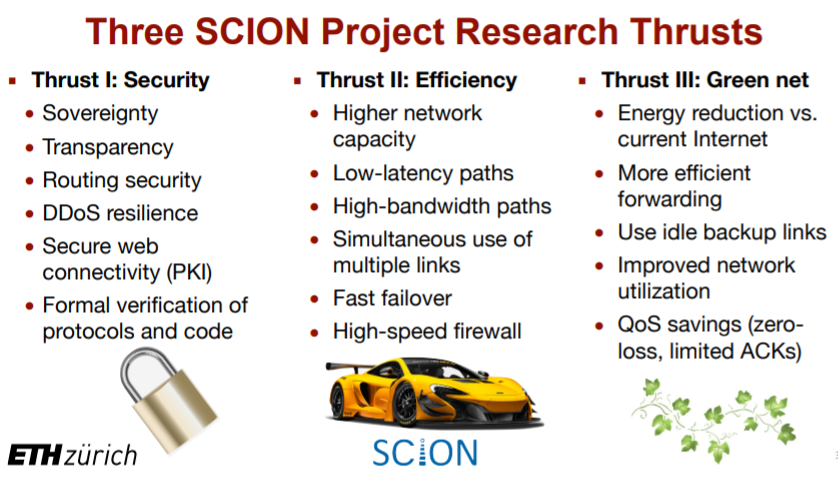
\includegraphics[scale=0.7]{images/910-why.PNG}
	\caption{SCION goals / motivation.}
	\label{fig:why}
\end{figure}

\subsubsection{SCION Overview}

\paragraph{Isolation Domain (ISD)}
A grouping of autonomous systems. An ISD has a core consisting of ASes that manage it and provide global connectivity (upstream = reach core). Each ISD has a root of trust governing it (trust root configuration, TRC) and can thus function autonomously without external trust.

\paragraph{Control Plane}
Responsible for the routing mechanisms. In SCION, the control plane constructs (path exploration) and disseminates (upon sender request) path segments. Each AS contains border routers, beacon servers and path servers. The control plane is also responsible for the dissemination and renewal of certificates needed to verify segments.

\textbf{Intra-ISD Path Exploration:} Done with beaconing. The core ASes initiate path-segment construction beacons (PCBs) which are flooded throughout the entire ISD - downstream ASes learn how to reach core ASes through the paths that the PCBs have taken (on the way down, each AS that sees the PCB appends itself as a next hop, additional to a MAC and its signature).

\textbf{Inter-ISD Path Exploration:} Same concept, just a lot denser than in the intra case. PCBs are distributed only among core ASes to create core-path segments.

\textbf{Path Server Infrastructure:} Path servers offer a lookup service (similar to DNS) to find down-path, up-path and core-path segments. The core ASes of each ISD operate the core-path and down-path server infrastructure (consistent and replicated) - selected path segments are chosen, stored and announced globally. Each non-core AS runs local path servers that serve selected up-path segments to local clients (no global announcements) along with resolving and caching responses of remote AS lookups.

In total, a host fetches the local up-path segments, global down-path segments and core-path segments if needed (to connect up- and down-path segments) by contacting its local path server with (ISD, AS) which might contact more path servers if info is not cached - this created an end-to-end path (which might be shorter than all segments combined - see yellow paths in Figure \ref{fig:paths}).

\begin{figure}[h]
	\centering
	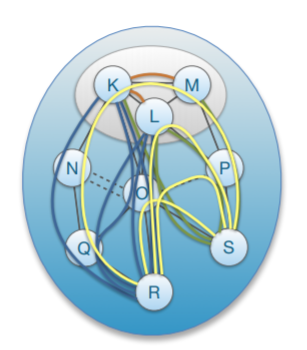
\includegraphics[scale=0.7]{images/910-path.PNG}
	\caption{Possible end-to-end paths from AS R to AS S (in yellow).}
	\label{fig:paths}
\end{figure}

\textbf{Path Combinations:} Not all path combinations are feasible due to security reasons. See Figure \ref{fig:combis} for all possible combinations.

\begin{figure}[h]
	\centering
	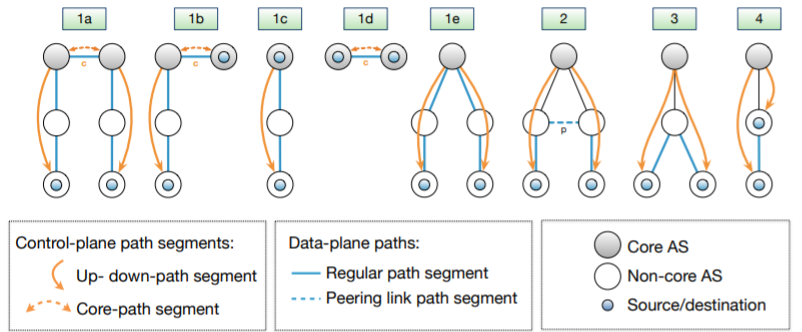
\includegraphics[scale=0.8]{images/910-combis.PNG}
	\caption{All possible ways to combine path segments.}
	\label{fig:combis}
\end{figure}

\paragraph{Data Plane}
Responsible for the actual packet forwarding. Path segments are combined to form a path. Segments (plus some metadata like geographical location or link latency) are included in the packet header (encrypted), therefore a sender knows exactly which ASes are traversed. A router only verifies the authenticity of the information (two AES operations replace longest-prefix match).


\paragraph{SCION Drawbacks}

\begin{itemize}
    \item Initial latency inflation to obtain paths during lookup (amortized by caching and path reuse since most destinations are reused).
    \item Bandwidth overhead due to paths in the packet headers - around 80 additional bytes (but enables path control and a simpler data plane).
    \item Increased complexity in key management due to new certificates like TRC certificates (necessary for a high security design).
    \item Initial set-up cost due to training network operators and installing new infrastructure (methods exist to facilitate deployment and new properties become possible with it).
\end{itemize}

\paragraph{SCION Deployment}
Since the AS infrastructure inside an ISP is being reused, there is not a lot of change necessary in the internal network infrastructure. We just need to set up core routers at the borders of an ISP (peering with other SCION-enabled networks and collect customer accesses). For end domains, we just need a SCION IP gateway (SIG) that enables seamless integration of SCION capabilities in end-domain networks. SIGs are then connected to SCION (border) routers. No upgrades of end hosts / applications are needed, it's just an additional packet header.

Incremental deployment is possible. Important to not rely on BGP for inter-domain operation s.t. we don't inherit its vulnerabilities. For local communication, intra-domain network architecture can be reused (intra-domain routing).


\subsubsection{SCION Security Insights}

\paragraph{Global Communication Guarantees}
Especially in the presence of adversaries. Goal: if a (routing policy compliant) path of good ASes exist, a sender can find, use and achieve minimum bandwidth guaranteed on that path. Challenges include: network routing instabilities / misconfigurations and DoS attacks are various levels (control and data plance, end hosts, etc.).

\textbf{Stable Forwarding and Multi-Path:} for the first challenge, these two concepts are necessary. Single-path forwarding cannot achieve strong availability guarantees (convergence, equipment failure, packet loss - path available / connectivity but shitty and needs manual intervention, etc.). With stable forwarding we have packet-carried forwarding state that protects forwarding from routing instabilities. With multi-path, we ensure the presence of several paths and as long as one works, end-to-end connectivity is assured. Overhead is low with the path segment combination method (instead of full paths). But, secure routing is insufficient in the case of outages caused by bottleneck links or continuing announcement of failed / congested routes since announcements in these cases are still legitimate.

\textbf{DoS Attacks:} SCION has several components that guarantee strong security and high availability (see Figure \ref{fig:secure}).

\begin{figure}[h]
	\centering
	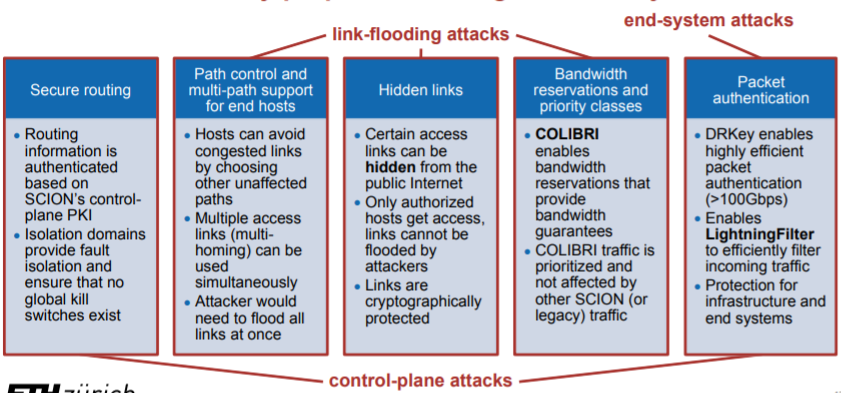
\includegraphics[scale=0.8]{images/910-secure.PNG}
	\caption{SCION protecting against DoS type attacks.}
	\label{fig:secure}
\end{figure}

\paragraph{High-Speed Packet Processing}
If you do it right, cryptographic operations can be performed on a per-packet basis. E.g. with a 400 Gbps link, a 64-byte packet arrives every 1.3ns. Symmetric crypto enables high-speed processing through parallel processing and pipelining - e.g. taking only around 100$\mu$s per signature (compared to a DRAM memory lookup that takes around 70ns). Not possible with asymmetric crypto. %TODO more here?

SCION offers a global framework for authentication and key establishment for secure network operations. DRKey = dynamically recreatable keys - creating crypto keys on the fly (within 20ns). With DRKey and EPIC, per-packet source authentication in software possible under 100ns. Control-plane PKI means that every AS has a public-key certificate that enables AS authentication and for each ISD to operate in a sovereign manner.

\textbf{DRKey:} use a per-AS secret value to derive keys with an efficient pseudo-random function (AES operation). With the secret value, a key created for another AS can be derived (fast) but without it (other AS) the key has to be fetched by contacting a local key server.

\textbf{Key Server Infrastructure:} each AS has a key server building the backbone of the key hierarchy. Servers are responsible for key exchange, management and local key establishment. After establishing AS-level keys, symmetric keys for end hosts can be provided and used to provide source authenticity of packets (without a costly key exchange). Each host is required to contact their local key server. See notes for a better explanation. %TODO example SCMP (exercise 13 as well), below

\textbf{LightningFilter:} SCION firewall that authenticates packets at very low overhead (no FP/FN, no heuristics). Sender locally fetches remote LightningFilter's DRKey and the filter then authenticates packets by deriving the DRKey. Normal to combine it with normal firewall (LF at border and firewall closer to destination). Also allows for history-based filtering by keeping track of rate of key requests of AS (and blocks if they overshoot). And duplicate suppression with bloom filters.

\textbf{EPIC: Every Packet Is Checked:} per-packet source authentication by every router and destination - possible with DRKey and a per-packet unique hop field (no duplication possible). Assumes global time synchronization. Same as in LF, source needs to first fetch all the keys to compute per-hop fields. Prevents malicious router replays / amplification and MAC bruteforce. %TODO hm, esp hop field thingy

%TODO comparisons with BGP / results at end of lecture

\paragraph{COLIBRI}
Provides practical and scalable global QoS. Stable paths that ensure reservations are not affected by routing changes. Multi-path system to search for paths with sufficient bandwidth. No per-flow state on routers (enables scalability) - possible with DRKey (per-packet source authentication), probabilistic large flow detection to detect overuse, per-flow stateful control-plane (server infra). Per-neighbor fairness (admission decision, ISP configs). %TODO ?? reservation?

\textbf{Admission Algo with Per-Neighbor Fairness:} instead of per-flow fairness (normal Internet), we have per-neighbor fairness. Each AS defines N2N minimum bandwidth guarantees (that can be computed for any path). Algo guarantees that no set of ASes can reserve a disproportionate amoung of bandwidth through any link. %TODO: example, how to compute??

\paragraph{Bandwidth Reservation}
Simplifies transport layer due to no need for sophisticated congestion control (simply use constant bitrate - good for streaming traffic). Low loss rate - low amount of ACKs. Enforce fairness at level of admissions. Traffic engineering.

%TODO scion vs. ip and bgp (exercise 13 and lecture)


